\label{Chapter5}
\chapter{Parallelisation} % Write in your own chapter title
\lhead{Chapter 5. \emph{Parallelisation}} % Write in your own chapter title to set the page header

[[ Introduction goes here ]]
The weak form of Maxwells equations means that parallelisation strategies are possibile.

The Message Passing Interface (MPI) is used and a *** strategy with distributed memory is utilised. The parallel computation is performed by a process of data decomposition. This means that the computational domain is partitioned into regions of space and each processor performs computations only on the elements in that region. This is made possible by the form of the weak form given in \eqref{maxwell-DG-weak-form}. We note that the weak form involves primarily values of unknowns on a single element. The only exception being the values of the solution $U_{out}$ from neighbouring elements required for the calculation of the numerical flux, $\tilde{\mathbf{F}}_n$ along element faces. These values should be made available to each element by communication between processors at each timestep.

\section{Update Equations in Parallel}

Let us consider calculation of updated solution values, $U^{n+1}_i$, from solution values at the previous timestep, $U^{n}_i$ for an element $\Omega_i$. Assume that the open bounded domain $\Omega \subset \R^{n}$ with boundary $\partial \Omega$ is partitioned with a regular partitioning in the usual way for finite elements as $\bar{\Omega} = \cup_{e} \bar{\Omega}_e$, such that $\Omega_i \cap􏰰\Omega_j = \O$, for $i \ne j$. The boundary $\partial \Omega$ is given by $\partial \Omega = \Gamma^{PEC} \cup \Gamma^{ABC}$ where $\Gamma^{PEC}$ and $\Gamma^{ABC}$ are repectively the boundaries along which PEC and ABC boundary conditions are prescribed and $\Gamma^{PEC} \cap \Gamma^{ABC} = \O$. We define the internal faces of the domain as $\Gamma^{I} = ( \cup_e \partial \Omega_{e}) \ \partial \Omega$.
We wish to divide the computational load between processors, by assigning calculations of each element to different processors. We define a regular partioning of $\Omega$ as $\bar{\Omega} = \cup_{p} \bar{\Omega}^p$ with partition boundary $\partial \Omega^{p}$. Each non-overlapping partition $\Omega^p$ is composed of a number of elements such that $\bar{\Omega}^p = \cup_{e} \bar{\Omega}_e$ and $\Omega^i \cap \Omega^j = \O$, for $i \ne j$. Parallelisation is achieved by assigning computation of the values $U^{n+1}_i$ from $U^{n}$ for each element $\Omega_e \in \Omega^p$ to a processor $P^p$.

For an element $\Omega_e \in \Omega^p$ we can define its adjacent elements, that is elements that share a face or edge, as $A_e = \{ \Omega_a \subset \Omega \| \partial \bar{\Omega}_a \cap \partial \bar{\Omega_e} \ne \O \}$. In general $A_e$ is composed of internal adjacent elements, $A_e^{int}$ = \{ A_e \cap \Omega^p \}, and external adjacent elements, $A_e^{ext} = \{ A_e \cap \Omega \setminus \Omega^p \}$. If $A_e^{ext} = \O$ the element $\Omega_e \in \Omega^p$ is said to be an internal element of $P^p$, and when $A_e{ext} \ne \O$ is said to be an interface element of $P^p$.An element $\Omega_e \in \Omega \setminus \Omega^p$ is said to be an external element of $P^p$.


Each element requires nodal values of $U_i^{n}$ from each of its adjacent elements only along shared faces (or edges). However in order to simplify the implementation, all nodal values of the solution of adjacent elements is communicated to the element in question at every time step. In this case the same data structures and conventions as outlined in Chapter [***] can be used to store the nodal values from other processors - which simplifies treatment in the code. This will incur a small performance penalty, however, for two processors containing a single triangle each with planar edges and linear shape functions communication was found to be only **** percent of total calculation time. This is expected to be an extreme case where computation greatly exceeds calculation time. However more realistic systems such as **** communication was only *** percent.

If the element $\Omega_e \in \Omega^p$ is an internal elements of $P^p$ all of the values of $U_i^n$ required to calculate $U_i^{n+1}$ are available on the processor $P^p$ from calculations on the previous timestep. However, if $\Omega_e$ is an interface elements, some of the values of $U_i^{n}$ will be available from calculations on $P^p$ for elements $A_e^{int}$, but will have been calculated on another processor on $A_e^{ext}$. At each time step, prior to face calculations, values of $U_i^{n}$ for elements in $A_e^{int}$ will be required on $P^p$, and should be sent to by each processor to which any element in $A_e^{int}$ is assigned. Or conversely, for each interface element, $\Omega_i$ in processor $P^p$, updated values of $U_n^i$ should be sent to any processors containing any element in $\A_e^{ext}$.

% maybe define what an adjacent processor of an ELEMENT is - that could help
% mention when U_out need to be available? Prior to compution. U_out calc prev time step.
% I've not mentioned (really) any correspondence between L^p_{out} and L^p_{in}
% talk about types of these elements and illustrate further with examples (figures)
% this could also be done as \Omega_i \subset L^p_{out} ?? How to I say that 

\section{Domain decomposition}

Since communication is an expensive operation with a significant overhead associated with each connection established we wish to minimise both the number of connections established and the information communicated at each time step. The number of messages can be significantly reduced by sending all values of $U_{n}$ once at the end of each time step.
% how much overhead? How expensive? What is more important? Communication of Computation?
Additionally we wish to choose $\Omega^p$ such that we minimise the number of processors which are required to communicate with each other, the volume of data which needs to be sent and the number of connections which needs to be established.
% *** is the number of connections ACTUALLY a different thing?
% *** at a later date I could also minimise the number of unknowns to communicate by weightng ( that comes under volume of data)


The three criteria can be met, if all elements have the same number of unknowns, by minimising the total number of external adjacent elements of all elements. This is equivalent to minimising the number of faces with in which the elements are on different processors. This operation can be performed by the public-domain library parMETIS [***], which implements several algorithms for the optimal partitionining of graphs.

% other processor has to know who they're from!! Talk about this in implementation
faces)
The parMETIS library requires a graph of the connectivities of all elements, in which each node of the graph represents an element and each edge of the graph represents a face shared between two elements. Since partitioning of the graph is performed in parallel the graph is given in a distributed data format in which each processor contains only a subset of the graph defined by a range of element indicies. The parMETIS library the accepts as a first parameter which specifies these ranges as an array which specifies for each processor the the first element index in its range. The last element index is then the element before the first element assigned to the next processor. The elements were distributed between processors equally, and the global element numbering established in the mesh file was used as a common numbering scheme between processors without need of communication.
A more optimal partitioning could be achieved if required by considering the type of each element and therefore the maximum number of shared faces, this however would require communication between processors in order to establish a common element indexing which is sequential within each processor. This would add significant to the complexity to the code and was not required for the problems which were considered.
% [*** not start points ? *** ]

The vertices of the graph are obtained by first constructing a node connectivity list, which for each node lists the elements which contain that node. This list is constructed by reading the whole mesh connectivity information and associating each read element which all the nodes it contains. The connectivites for all elements is read - however since these are integer values memory usage is not considered relevant [ *** give an example of a very large mesh]. We loop through all faces of the elements allocated to this processor and for each face perform a loop on the nodes within that face. Within the inner loop we construct a list of connected elements [what is this]. The connected face will be the element in this list which appears the same number of times as the number of nodes in the face.

From the connectivity graph, parMETIS can then optimise the partitions in such a way to reduce the number of faces shared across processors. The resulting partition is shown for a circle with 5 processors in \figref{parmetis-figure}

The result of the optimisation by parMETIS is a list of all elements allocated to this processor and a number between 1 and the total number of processors (or equivalently the number of parts into which the domain is partitioned) which indicated the processor on which calculations should be performed (or equivalently the parition in which this element belongs). We allow each partition of the domain to correspond to a partitioning $\Omega^p$.

\section{Communication Arrays and Data Partition}

Recall that in order to implement the parallelised DG method it is not sufficient to distribute computations, some values of solution need to be communicated at each time step. In order to simplify the extension of a serial code to multiple processors the strategy employed involves establishing the set of elements that, for a given processor $A$, share a face with an element in the partition allocated to processor $A$. All nodal solution values for these elements are mirrored from the processor on which they are calculated to processor $A$ at each time step. The data partition is show in \figref{parmetis-figure} and results in a number local elements on which calculations are performed on this processor and a number of interface elements for which nodal solution values are available without calculation. By this data partition method code to calculate the numerical flux contributions does not need to distinguish betweeen local elements and interface elements. The advantage of this method is that the elements allocated to a processor and the interface elements can be stored in the same data structures.

Once the partitioning has been performed parMETIS provides a list of partition numbers, the length of the number of elements in the partition range of this processor. The partition numbers correspond to the processor partition $\Omega^p$, to which the given element should be allocated for calculation. In order to set up communication arrays additional information is required. For each element allocated to a partition $P$ the elements to which it is connected are required, which is available on the current partition, and also a list of the processors on which the element will the allocated for calculation. These eventual destinations are obtained for each element by MPI communication following partitioning. Then for each element the global index of the element and a list of the global indexes of its adjacent elements which are not on the destination processor and for each of those adjacent elements the processor on which they will be located is sent to the processor on which communication will occur.

Each processor will therefore recieve from all processors a list of the elements that are allocated to that processor and also a list of the elements to which those elements are connected. Note that in this instance the processor is sending information to itself via MPI, but this will not incur a communication overhead. From this information a list of all the elements on this processors for which calculations will occur, or local elements, can be constructed and also a list of all elements which are connected by a shared face one or more times to this processor, the non-local elements. The mesh connectivity information can then be re-read for all elements (both local and non-local) and coordinates of mesh vertices are required for local elements. The code may then proceed exactly as in the serial case but only looping over the local elements for calculations. The only difference is that following each solution update communication should occur to update the nodal in the interface elements based on the elements in the other processor.

% NEXT: HOW DO WE SET UP THE COMMUNICATION ARRAYS - I'VE GOT THE ELEMENTS ON EACH PROCESSOR NOW - BUT I NEED LOOP THROUGH ALL OF THESE AND SET UP COMMS ARRAYS BASED ON THE DESTINATION PROCESSOR OF CONNECTED ELEMENTS.


The mesh can then be re-readThe mesh data required (both for the local and non-local elements) can then be constructed. This is done by constructing a unique list of the elements which

The communication arrays are required

** I need to talk here about how I set up the communication arrays, what else needs doing? what communication is required in pre-processing stage? etc **
** question: why do I need to keep track of the original numbering scheme? (i.e. localElementMap) **

\begin{figure}[htbp!]
 \centering
 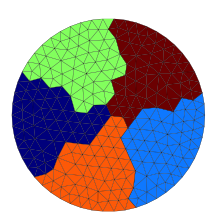
\includegraphics[width=0.3\textwidth]{Figures/Parallelisation/parmetisPartition}
 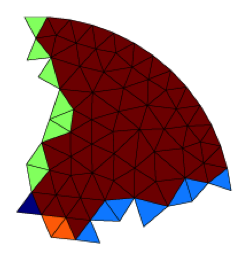
\includegraphics[width=0.2\textwidth]{Figures/Parallelisation/parmetisDataPartition}
\caption{Left: Partition of a circle given by parMETIS. Each color represents a different processor on which calculations for that processor should be performed. Right: Data partition of elements for a single processor (red) for circle}
\label{parmetis-figure}
\end{figure}

The nodal values to communicate between processors is be established in the preprocessing state, prior to computation. By parsing the graph and communication each processor recieves a list of elements for computation and the processors to which their nodal values should be sent and a list of interface elements ordered by processors number on which calculations occur. The vector of unknowns $U$, is implemented as a 1-dimensional array. By using the sendtoall functions available through the MPI library the elements numbering can be done in such a way that the MPI buffer recieved is a contiguous section of the vector U. this removes the need for a map of nodal values or copying values between the MPI buffer and the vector $U$.

The solution can be advanced in time following the exact procedure as the serial code, for a single partition of the domain per processor, provided that at each stage of the RK4 method the the nodal solution values should are communicated.

\section{Ordering of Faces}
